% % % % % % % % % % % % % % % % % % % % % % % % % % % % % % % % % %
%  Devolutiva — Fase 1: Imersão
%  Disciplina: Design Thinking (DE_233) — ETE Cícero Dias
%  Profa. Samara Silva  ·  Recife, 19 de junho de 2026
% % % % % % % % % % % % % % % % % % % % % % % % % % % % % % % % % %

\documentclass[
  sigconf,
  nonacm, % Remove o rodapé da ACM
  language=portuguese
]{acmart}

% ── Desliga rodapé ACM ──────────────────────────────────────
\settopmatter{printacmref=false}
\setcopyright{none}
\acmYear{2026}
\let\balance\relax

% ── Mata a página temporária da ACM (compilação única via API) ──
\makeatletter
\def\acm@addtemp@page{}
\makeatother

% ── Pacotes ─────────────────────────────────────────────────
\usepackage[portuguese]{babel}
\usepackage{microtype}
\usepackage{booktabs}
\usepackage{tabularx}
\usepackage{array}
\usepackage{colortbl}
\usepackage[dvipsnames,table]{xcolor}
\usepackage[inline]{enumitem}
\usepackage{graphicx}
\usepackage{adjustbox}
\usepackage{fancyhdr}
\usepackage{eso-pic} % Para a capa preencher toda a página sem gerar páginas em branco

% ── Ajuste contra quebras de texto ruins (Textos Cortados) ──
\tolerance=1000
\emergencystretch=1.5em

% ── Cores ───────────────────────────────────────────────────
\definecolor{cgood}{HTML}{1E6B3A}
\definecolor{cwarn}{HTML}{8B4500}
\definecolor{cred}{HTML}{C0392B}
\definecolor{cmuted}{HTML}{666666}
\definecolor{crow}{HTML}{F2EFEB}

% ── Colunas customizadas para tabela ────────────────────────
\newcolumntype{L}[1]{>{\raggedright\arraybackslash}p{#1}}
\newcolumntype{C}[1]{>{\centering\arraybackslash}p{#1}}

% ── Comando nota destacada ───────────────────────────────────
\newcommand{\notadestaque}[2]{%
  \noindent\textbf{Nota:}\enspace%
  {\large\bfseries\color{cred}#1\,/\,#2\,pts}%
}

% ── Comando label de status ──────────────────────────────────
\newcommand{\statusok}[1]{{\small\bfseries\color{cgood}#1}}
\newcommand{\statuswarn}[1]{{\small\bfseries\color{cwarn}#1}}

% ── Renomeações PT-BR ────────────────────────────────────────
\AtBeginDocument{%
  \renewcommand{\abstractname}{Resumo}
  \renewcommand{\figurename}{Figura}
  \renewcommand{\tablename}{Tabela}
}

% ────────────────────────────────────────────────────────────
\begin{document}

% ── CAPA ────────────────────────────────────────────────────
\thispagestyle{empty}
\AddToShipoutPictureBG*{%
  \AtPageLowerLeft{%
    \IfFileExists{capa.png}{%
      
\includegraphics[width=\paperwidth,height=\paperheight]{capa.png}%
    }{%
      \IfFileExists{../../capa.png}{%
        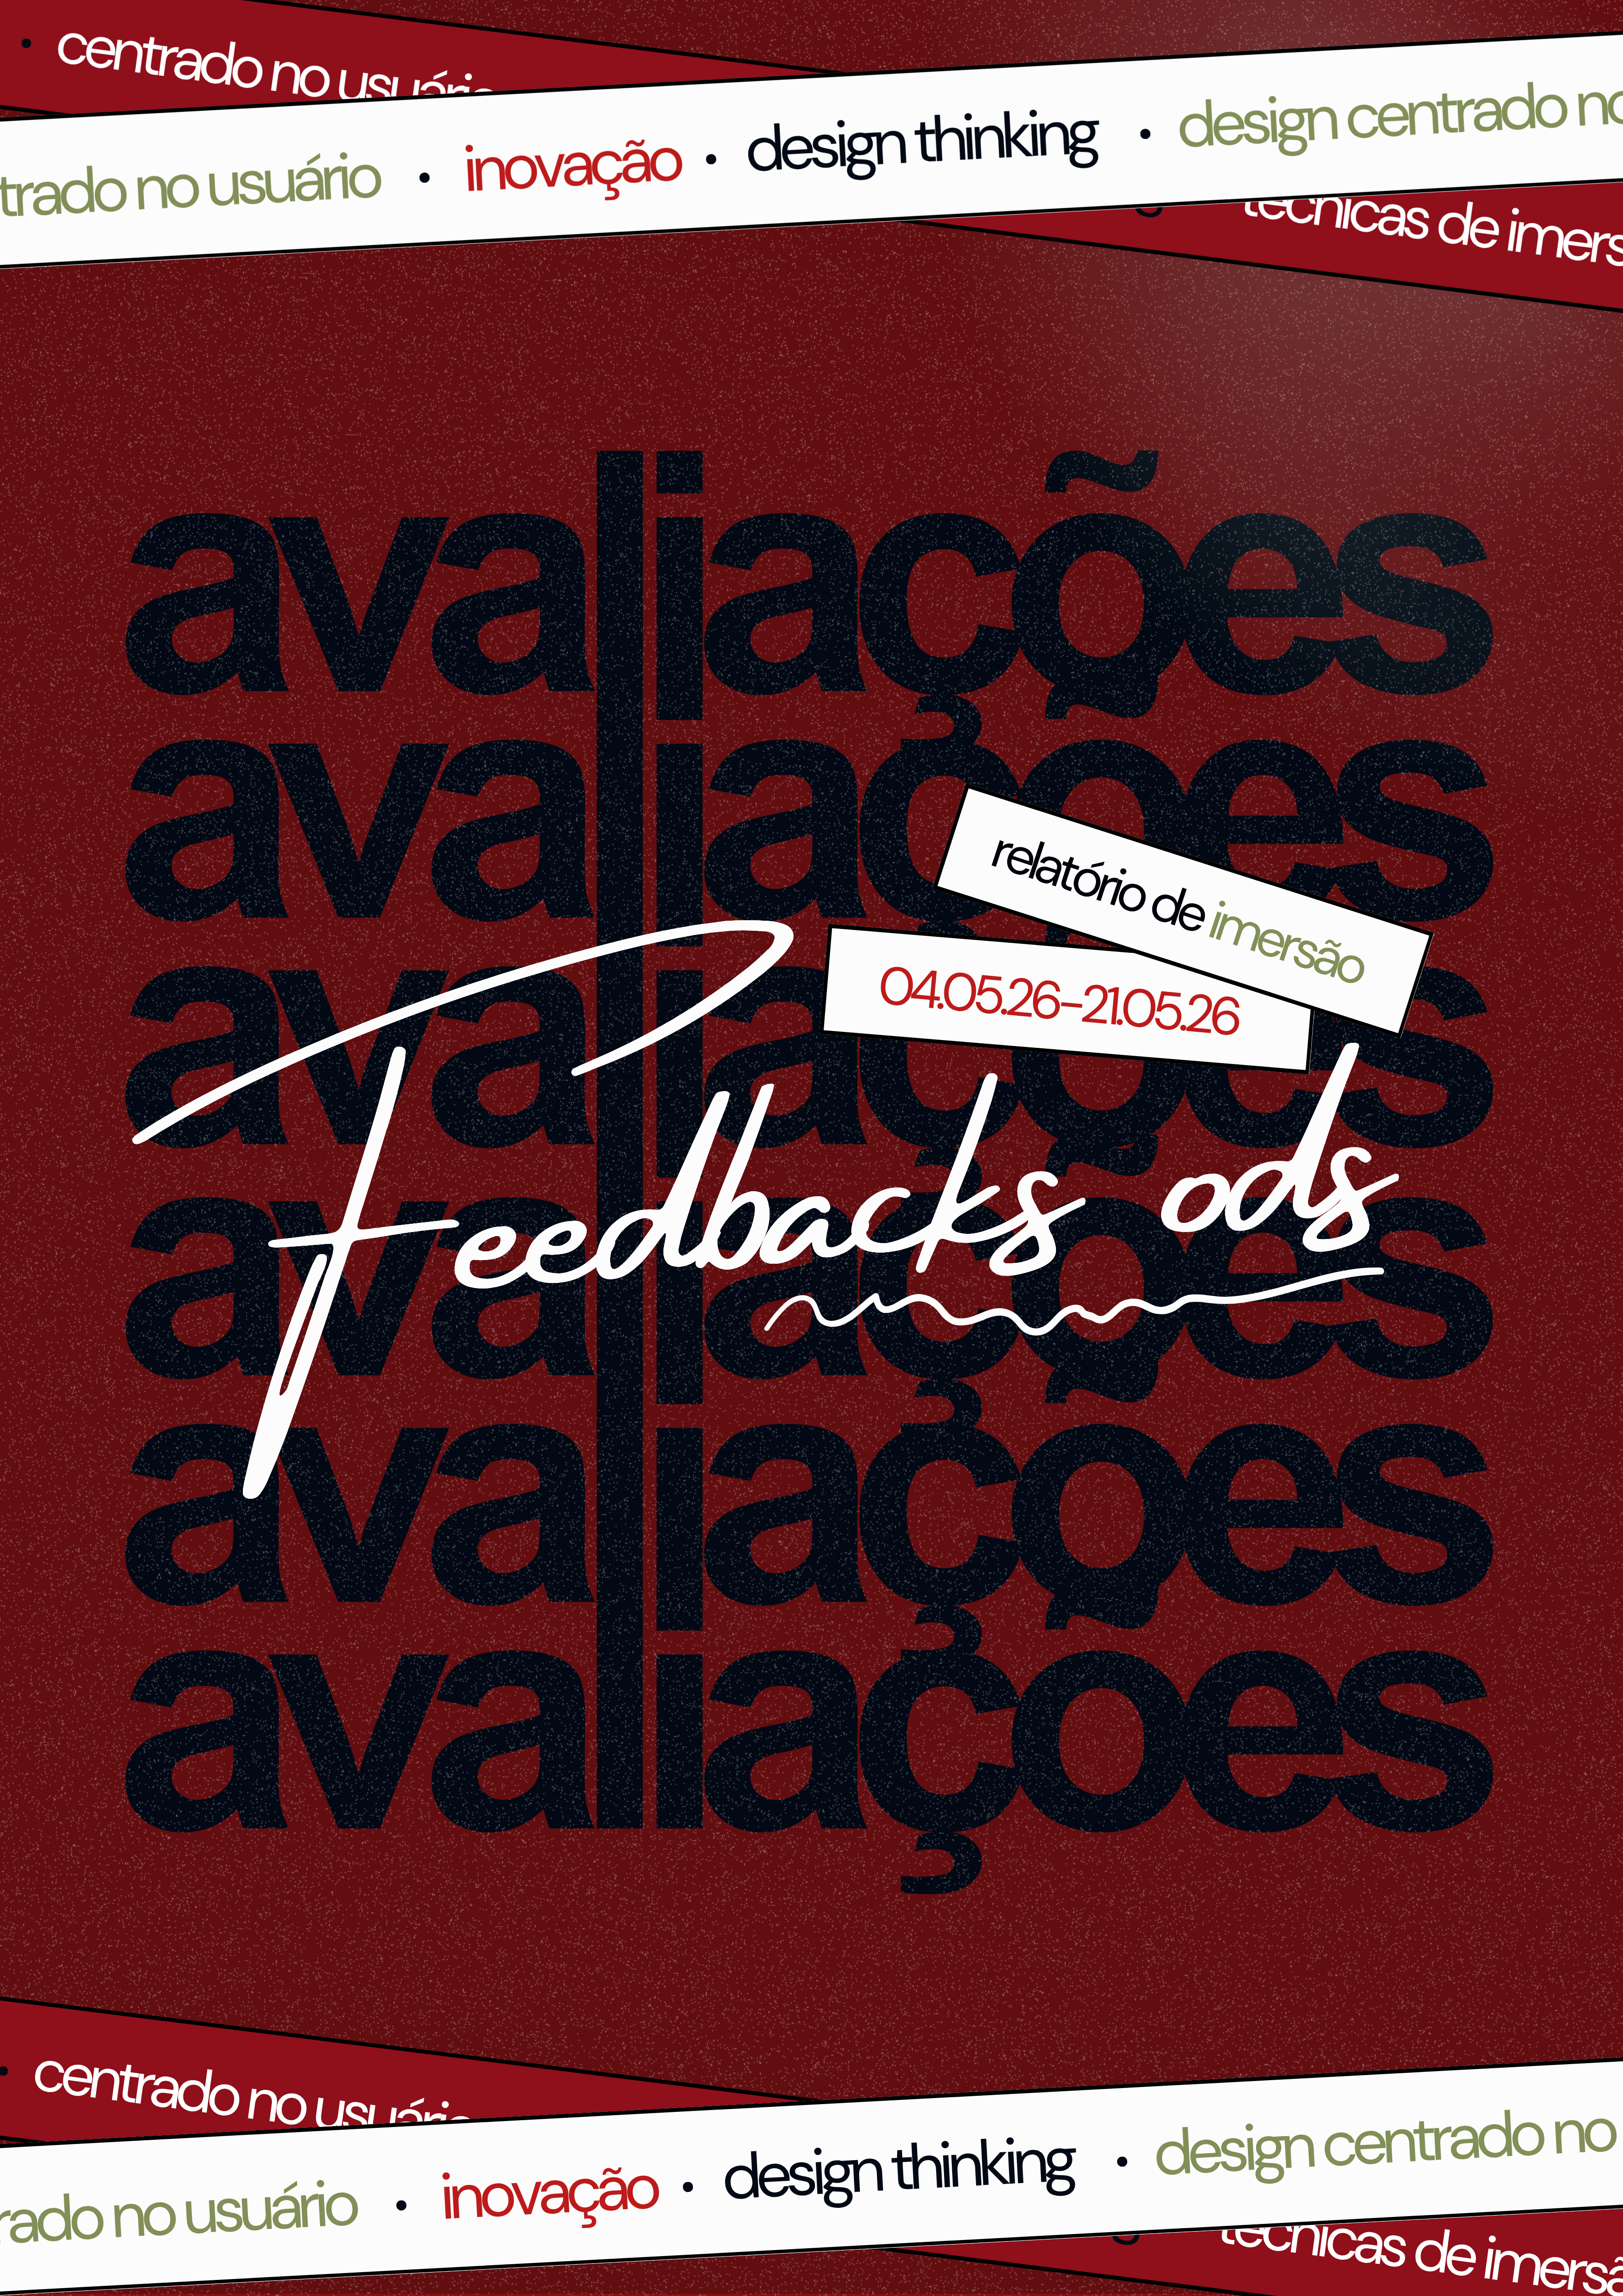
\includegraphics[width=\paperwidth,height=\paperheight]{../../capa.png}%
      }{%
        \parbox[b][\paperheight]{\paperwidth}{%
          \vspace*{10cm}\begin{center}{\large\color{gray}[capa.png não encontrada]}\end{center}%
        }%
      }%
    }%
  }%
}
\mbox{} % Caixa vazia para garantir que a página da capa seja gerada e preenchida
\clearpage

% ── CONFIGURAÇÃO DE PÁGINA PÓS-CAPA ─────────────────────────
\setcounter{page}{1}
\pagestyle{fancy}
\fancyhf{}
\renewcommand{\headrulewidth}{0pt}
\fancyfoot[C]{\thepage}
\setlength{\headsep}{0.8cm} % Distancia o cabeçalho do conteúdo das colunas

% ── METADADOS ────────────────────────────────────────────────
\title{Feedback Avaliativo de Projeto: Design Centrado no Usuário --- Fase 3 — Ideação (lente DCU)}

\author{Profa.\ Samara Silva}
\authornote{Grupo: \textbf{Grupo 01 - Fome Zero} \textperiodcentered\ Per\'{i}odo: 22 de maio de 2026 \textperiodcentered\ Avaliado em: 19 de junho de 2026.}
\email{samarasilvia.educa@gmail.com}
\affiliation{%
  \institution{ETE C\'{i}cero Dias}
  \department{M\'{o}dulo 1 --- Turma A · 2026.1}
  \city{Recife}
  \state{Pernambuco}
  \country{Brasil}
}

\author{Grupo 01 - Fome Zero}
\affiliation{%
  \institution{ETE C\'{i}cero Dias}
  \department{Turma --- Turma A · 2026.1}
  \city{Recife}
  \state{Pernambuco}
  \country{Brasil}
}
\maketitle

\vspace{1em}
\section{Avaliação Geral}

\notadestaque{0,00}{5,00}

A avaliação foi concluída. A seguir o resumo dos critérios e os comentários detalhados.

\subsection{Resumo dos Critérios}

\rowcolors{2}{crow}{white}
\begin{tabular}{@{} L{2.6cm} C{2.5cm} C{1.1cm} C{1.1cm} @{}}
\toprule
\textbf{Critério} & \textbf{Status} & \textbf{Nota} & \textbf{Máx.} \\
\midrule
Solução Centrada no Usuário & \statuswarn{Não entregue} & \textbf{0,00} & 2,00 \\
Jornada do Usuário AS TO BE — Qualidade UX & \statuswarn{Não entregue} & \textbf{0,00} & 2,00 \\
Documentos de Ideação — Clareza Visual & \statuswarn{Não entregue} & \textbf{0,00} & 1,00 \\
\midrule
\textbf{Total} & & \textbf{\color{cred}0,00} & \textbf{5,00} \\
\bottomrule
\end{tabular}

\section{Comentários por Critério}

\subsection{Solução Centrada no Usuário}

\noindent\statuswarn{0,00\,/\,2,00 pts · Não entregue}

\begin{itemize}[leftmargin=14pt,itemsep=1pt,topsep=3pt,parsep=0pt]
  \item[$\square$] {\small\textcolor{cmuted}{A solução responde diretamente às dores da persona}}
  \item[$\square$] {\small\textcolor{cmuted}{As decisões de ideação são justificadas pelo usuário, não por preferência do grupo}}
  \item[$\square$] {\small\textcolor{cmuted}{Há conexão clara entre o problema do usuário e a solução proposta}}
  \item[$\square$] {\small\textcolor{cmuted}{As funcionalidades descritas atendem a dores e necessidades concretas da persona}}
  \item[$\square$] {\small\textcolor{cmuted}{Cada funcionalidade tem justificativa centrada no usuário — fica claro por que ela existe}}
  \item[$\square$] {\small\textcolor{cmuted}{A descrição evidencia como o usuário interage com a solução e o que ganha em cada etapa}}
  \item[$\square$] {\small\textcolor{cmuted}{Mostra como a solução melhora a experiência em relação à jornada atual}}
\end{itemize}

\subsection{Jornada do Usuário AS TO BE — Qualidade UX}

\noindent\statuswarn{0,00\,/\,2,00 pts · Não entregue}

\begin{itemize}[leftmargin=14pt,itemsep=1pt,topsep=3pt,parsep=0pt]
  \item[$\square$] {\small\textcolor{cmuted}{Aponta onde a solução resolve as dores mapeadas}}
  \item[$\square$] {\small\textcolor{cmuted}{O contraste entre a jornada atual e a futura está visível e legível}}
  \item[$\square$] {\small\textcolor{cmuted}{A jornada é diagramada com clareza: etapas, pontos de contato e hierarquia visual}}
  \item[$\square$] {\small\textcolor{cmuted}{Indica o estado emocional do usuário ao longo das etapas}}
\end{itemize}

\subsection{Documentos de Ideação — Clareza Visual}

\noindent\statuswarn{0,00\,/\,1,00 pts · Não entregue}

\begin{itemize}[leftmargin=14pt,itemsep=1pt,topsep=3pt,parsep=0pt]
  \item[$\square$] {\small\textcolor{cmuted}{Os documentos estão bem organizados e legíveis}}
  \item[$\square$] {\small\textcolor{cmuted}{Consistência visual entre os documentos — tipografia, cores e espaçamento}}
\end{itemize}

\section{Considerações Finais}

Os ajustes indicados são de natureza metodológica e devem ser
incorporados para as próximas entregas.
Continuem assim.

% ── Assinatura ───────────────────────────────────────────────

\vspace{1.5em}
\noindent\rule{\linewidth}{0.4pt}

\begin{flushright}
\textbf{Profa.\ Samara Silva}\\
{\small\color{cmuted} Design Thinking --- DE\_233 · ETE Cícero Dias}\\
{\small\color{cmuted} Recife, 19 de junho de 2026}
\end{flushright}

% ── Sem referências bibliográficas ───────────────────────────

\appendix
\onecolumn
\section{Critérios e Níveis de Avaliação}

Esta seção apresenta os critérios de avaliação para referência dos estudantes.

\subsection{Níveis de Completude}

\begin{tabularx}{\linewidth}{@{} p{4cm} p{1.5cm} X @{}}
\toprule
\textbf{Nível} & \textbf{\%} & \textbf{Descrição} \\
\midrule
Completo & 100\% & Fez tudo e fez certo. Critério plenamente atendido. \\
Completo c/ ressalvas & 85\% & Fez tudo, mas algo ficou incorreto ou impreciso. Esforço total, qualidade com falha. \\
Completo, mas inadequado & 70\% & Preencheu todos os itens, porém boa parte do conteúdo não atende ao propósito da atividade. \\
Faltou pouco & 65\% & Fez bastante e acertou o que fez. Faltaram partes, mas o que entregou presta. \\
Faltou pouco c/ erros & 60\% & Fez bastante, mas errou partes relevantes. Metade do caminho com qualidade irregular. \\
Faltou muito & 40\% & Fez pouco, mas o que fez está correto. Entrega incompleta, execução ok. \\
Faltou muito e errou & 25\% & Fez pouco e ainda errou. Esforço baixo, qualidade baixa. \\
Errado & 10\% & Tentou, mas a abordagem foi incorreta por completo. Reconhece a tentativa. \\
Não fez & 0\% & Critério não entregue. \\
\bottomrule
\end{tabularx}

\vspace{1em}
\subsection{Penalizações por Atraso}

\begin{tabularx}{0.6\linewidth}{@{} X p{5cm} @{}}
\toprule
\textbf{Atraso} & \textbf{Desconto} \\
\midrule
Até 1 dia & -10\% \\
2–3 dias & -20\% \\
Mais de 3 dias & -30\% \\
Não entregou & Zera a nota \\
\bottomrule
\end{tabularx}

\section{Devolutiva Individual}

A nota individual é calculada aplicando o fator de contribuição sobre a nota do grupo em cada fase.

\subsection{Fatores de Contribuição}

\begin{tabularx}{0.6\linewidth}{@{} X c @{}}
\toprule
\textbf{Fator} & \textbf{Multiplicador} \\
\midrule
Liderou & 100\% \\
Participou & 100\% \\
Participou pouco & 70\% \\
Só fez sua parte & 40\% \\
Não participou & 0\% \\
\bottomrule
\end{tabularx}

\vspace{1em}
\subsection{Notas por Integrante}

\begin{tabularx}{\linewidth}{@{} X X p{2.5cm} @{}}
\toprule
\textbf{Integrante} & \textbf{\small DCU Fase 3 — Ideação (lente DCU)} & \textbf{Total} \\
\midrule
André da Silva Durães & 0,00 \textit{(Não participou)} & \textbf{0,00} \\
Bruna Maria do Nascimento Costa & 0,00 \textit{(Não participou)} & \textbf{0,00} \\
João Gabriel Cavalcanti & 0,00 \textit{(Participou)} & \textbf{0,00} \\
Suammyr Cavalcante do Carmo & 0,00 \textit{(Liderou)} & \textbf{0,00} \\
Maria Zilda Ferreira Pinto & 0,00 \textit{(Participou)} & \textbf{0,00} \\
Ayran Gabriel Duque Souza Lima & 0,00 \textit{(Não participou)} & \textbf{0,00} \\
\bottomrule
\end{tabularx}

\end{document}
